\section{Introduction}


\paragraph{Motivation}
\begin{itemize}
    \item In recent years NN for image classification had a lot of successes.
    \item It's researches obligation to ensure NN robustness and reliability of NNs.
    \item It’s widely known fact that NN are vulnerable against adversarial attacks~\cite{ilyas2019adversarial}.
    \item Pretext tasks had shown themselves usefully to improve accuracy~\cite{kolesnikov2019revisiting}.
    \item In this research I would like to evaluate how including state-of-the-art pretext tasks in training
    process influences NNs vulnerability against adversarial attacks.
\end{itemize}

\subsection{Background and Related work}

\paragraph{Adversarial attack}
Goodfellow defined adversarial attacks as “inputs to machine learning models that an
attacker has intentionally designed to cause the model to make a mistake.” ~\cite{DBLP:journals/corr/abs-1802-08195} \\
In the domain of image classification, adversarial attacks are images usually formed by applying a small perturbation
(which is barely noticeable for human viewer) to a naturally occurring image, with intention to make NN miss-classify.

\paragraph{Fast gradient sign method}
The name was first introduced by Goodfellow and Jonathon Shlens and Christian Szegedy
~\cite{goodfellow2015explaining} as guaranteed approach to make artificial NN miss-classify an image,
which still would de be recognisable as of the same class for human viewer.
Fast gradient sign method (further denoted as FGSM) works by using the gradients of the neural network to create an adversarial pattern.
For an input image, the method evaluates the signed gradient of the loss function with respect to the input image to create a pattern,
which maximises the loss.
The pattern is then added pixel wise to original image.
The new image is called the adversarial image.
The process can be summarised using the following expression:
\begin{equation}
    adv\_x = x + \epsilon \cdot sign(\nabla_x J(\theta, x, y))
\end{equation}
(where $\epsilon$ denotes the intensity of adversarial pattern).
\\
\begin{figure}[h]
    \begin{subfigure}{0.4\textwidth}
        \caption{Tulips 40\% confidence}
        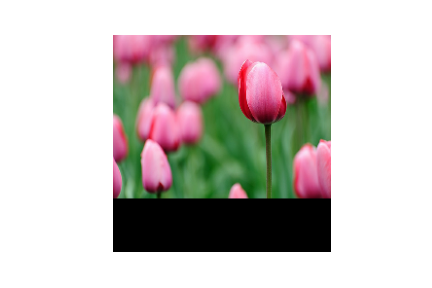
\includegraphics[width=8cm]{images/og_image}
    \end{subfigure}
    \begin{subfigure}{0.4\textwidth}
        \caption{Adversarial pattern for this image}
        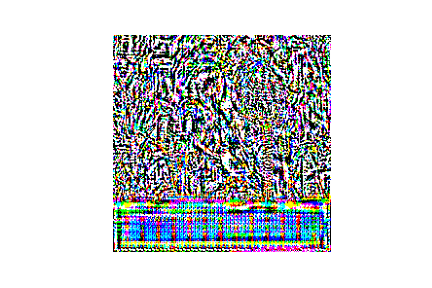
\includegraphics[width=8cm]{images/adv_pattern}
    \end{subfigure}
    \\
    \begin{subfigure}{0.4\textwidth}
        \caption{$\epsilon = 0.01$, Roses 40\% confidence}
        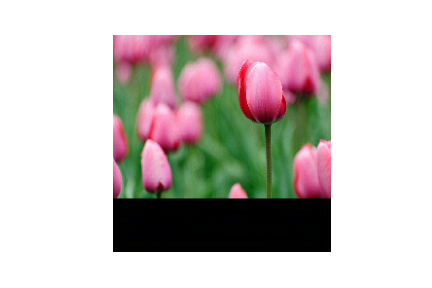
\includegraphics[width=8cm]{images/adv_attack_001}
    \end{subfigure}
    \begin{subfigure}{0.4\textwidth}
        \caption{$\epsilon = 0.1$, Roses 40\% confidence}
        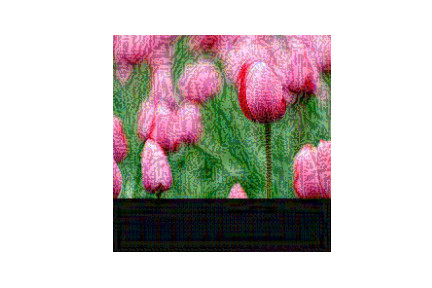
\includegraphics[width=8cm]{images/adv_attack_01}
    \end{subfigure}
\end{figure}

\paragraph{Pretext task}
Pretext task is the self-supervised learning task solved to learn visual representations,
with the aim of using the learned representations or model weights obtained in the process, for the downstream task.
It has been showm, that pretext tasks can significantly improve NNs accuracy.~\cite{kolesnikov2019revisiting}
It is also believed they contribute to NNs learning of important (as per human agents) features.

\paragraph{Efficient Net}
Convolutional networks' architectures for image recognition have evolved quite drastically in recent years, with numerous options available "out of the box".
A.e.Efficient Net (further denoted as EffNet) delivers impressive accuracy, while being able to scale better than a lot of previous architectures~\cite{DBLP:journals/corr/abs-1905-11946}.
All the evaluations were \st{done} using it, namely EfficientNetB0.

\paragraph{Rotation pretext task}
A common choice of pretext task could be to produce 4 copies of
a single image by rotating it by {0°, 90°, 180°, 270°} and let a single network predict the rotation which was applied.
~\cite{kolesnikov2019revisiting}
Intuitively, a good model should learn to recognize canonical orientations of objects in natural images."

\paragraph{Jigsaw pretext task}
The task is to recover relative spatial position of 4 sampled image patches after a random permutation of these patches was performed.
~\cite{kolesnikov2019revisiting}
All of these patches are concatenated in 'puzzle' image, which is later sent through same network, which needs to predict a permutation applied.


\section{Methods}


\paragraph{Rotation pretext task}
Each image from original dataset was rotated 0°,90°,180°,270° and assigned new pseudo label:
\begin{itemize}
    \item 0° \textrightarrow \; 0
    \item 90° \textrightarrow \; 1
    \item 180° \textrightarrow \; 2
    \item 270° \textrightarrow \; 3
\end{itemize}
all 4 batches of rotated images were concatenated in dataset, and shuffled.
Then last dense layer of NN was replaced with dense layer for corresponding number of pseudo classes (4).
Then same model was then trained to identify rotation applied.
\\
\begin{figure}[h]
    \begin{subfigure}{0.33\textwidth}
        \caption{Label = 0}
        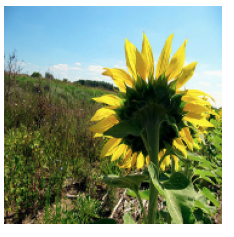
\includegraphics[width=5cm]{images/rot_0}
    \end{subfigure}
    \begin{subfigure}{0.2\textwidth}
        \caption{Label = 1}
        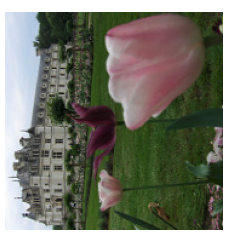
\includegraphics[width=5cm]{images/rot_1}
    \end{subfigure}
    \begin{subfigure}{0.33\textwidth}
        \caption{Label = 2}
        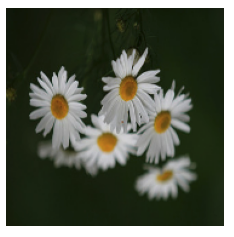
\includegraphics[width=5cm]{images/rot_2}
    \end{subfigure}
    \caption{An example how images used for rotation pretext task could look like}
\end{figure}

\paragraph{Jigsaw pretext task}
For jigsaw similar approach as described by Mehdi Noroozi and Paolo Favaro~\cite{DBLP:journals/corr/NorooziF16} was adopted.
Random 4 out of 24 possible permutations were chosen for each batch.
(number of possible permutation can be obtained from Newtonian binomial $P=\frac{r!}{(r-n)!}$).
For each permutation each image was cut in 4 equal parts, they were afterwards permuted according to chosen permutation,
and concatenated in 1 image afterwards.
For detailed implementation please refer to \href{https://github.com/Goofy-Goof/ISS/blob/33a2ad40b779ff230aae31c29d2edc2cf5d90406/impl/util/pretext.py}{GitHub/pretext.py}.
Similarly to rotation pseudo labels in [0\ldots23] have been assigned, images were shuffled and dense layer was replaced by suitable one.
The network then is trained to identify permutation applied.
\\
\begin{figure}[h]
    \begin{subfigure}{0.33\textwidth}
        \caption{Original image}
        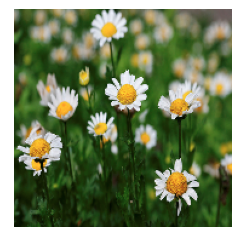
\includegraphics[width=5cm]{images/dandelion}
    \end{subfigure}
    \begin{subfigure}{0.2\textwidth}
        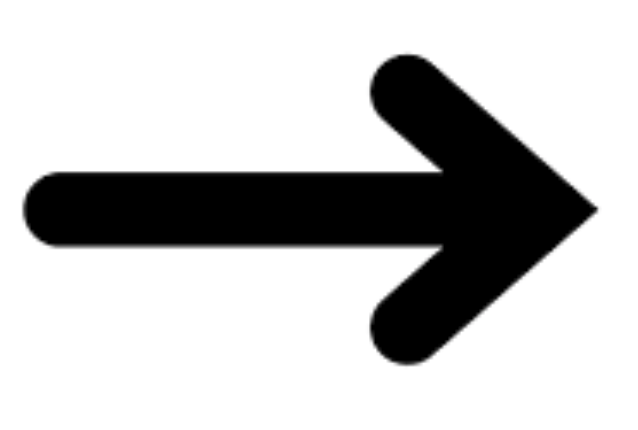
\includegraphics[width=3cm]{images/arrow}
    \end{subfigure}
    \begin{subfigure}{0.33\textwidth}
        \caption{Generated puzzle, label=1}
        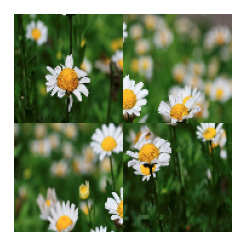
\includegraphics[width=5cm]{images/puzzle}
    \end{subfigure}
    \caption{An example how puzzle for jigsaw pretext task could look like}
\end{figure}

\paragraph{Adversarial Images with FGSM}
My implementation of FGSM was based on \href{https://www.tensorflow.org/tutorials/generative/adversarial_fgsm}{TF FGSM}.
In order to generate adversarial pattern for each image, gradient of loss function is evaluated with sign for each image.
Then according to this formula:
\begin{equation}
    adv\_x = x + \epsilon \cdot sign(\nabla_x J(\theta, x, y))
\end{equation}
pattern was then added pixel wise to original image with $\epsilon$ varying in [0.01\ldots0.1]
(any higher values make the image visually disrupted for human viewer).
Resulting adversarial image was then clipped by value, so each pixel value stays in interval [0\ldots255],
as required for RGB color encoding.
For detailed implementation please refer to \href{https://github.com/Goofy-Goof/ISS/blob/33a2ad40b779ff230aae31c29d2edc2cf5d90406/impl/util/adversarial.py}{GitHub/adversarial.py}


\paragraph{Evaluation approach}
In order to evaluate, how including pretext task in training process influences NNs vulnerability against adversarial attacks,
Intensity of adversarial pattern needed to make NN miss classify (Further denoted with epsilon or $\epsilon$) was measured.
\\
5\% of dataset were reserved for experiment.
During each evaluation round NN network was trained with rotation or jigsaw pretext task.
Number of training epochs was varied in [25, 50, 75, 100] for pretext training, Number of epochs for downstream training was set to 50.
\\
Reserved images were given to NN, the ones which were correctly classified saved.
Then for each of saved (previously correctly classified images) adversarial image was created using FGSM with $\epsilon = 0.01$.
If classification was still correct $\epsilon$ value was increased by 0.005.
This was repeated until NN produced false classification or $\epsilon$ reached value of 0.1
\\
$\overline{\epsilon}$ was compared for different values of pretext training epochs and kinds of pretext tasks.
In order to compare how pretext tasks perform in comparison with other popular state of the art pre-training technics perform,
the result were compared with EffNet trained for 50 epochs without pretext task and EffNet pre-trained for image classification on ImageNet.